\chapter{System Architecture and Design}\label{ch:architecture}

This chapter presents the complete system architecture of our privacy-preserving electronic voting system. We establish the design principles that guide all architectural decisions, describe the layered system structure, formally define the threat model, and detail the cryptographic protocols that enable simultaneous voter authentication and ballot privacy.

\section{Design Principles}

Five core principles govern every architectural and implementation decision in our system:

\begin{enumerate}[label=\textbf{P\arabic*}]
    \item \textbf{Zero-Knowledge Privacy}: No entity---including system operators, blockchain validators, or observers---can determine how a specific voter cast their ballot. The system achieves cryptographic unlinkability between voter identity and ballot content.
    
    \item \textbf{Trustless Verification}: All election results are independently verifiable from public on-chain data. No trusted third party (coordinator, mix-net server, or election authority) is required for correctness. Any observer can reconstruct the Merkle tree, re-verify all proofs, and recompute the tally.
    
    \item \textbf{Economic Inclusivity}: Voting must be free for all citizens regardless of economic status. The system eliminates gas fees through a sovereign blockchain with authority-sponsored execution, ensuring that financial barriers never prevent democratic participation.
    
    \item \textbf{Administrative Fidelity}: The system models the real Sri Lankan administrative hierarchy---Election Commission, 22 districts, 160 polling divisions, 14,000+ GN divisions---with on-chain role delegation. This is not a toy prototype; it reflects actual governance structures.
    
    \item \textbf{Defense in Depth}: Security does not rely on any single mechanism. Five independent layers of fraud prevention ensure that compromising one layer does not compromise the election. Each layer addresses a distinct attack vector.
\end{enumerate}

\section{System Architecture Overview}

The system follows a four-layer architecture, each with clear responsibilities and well-defined interfaces:

\begin{figure}[H]
\centering
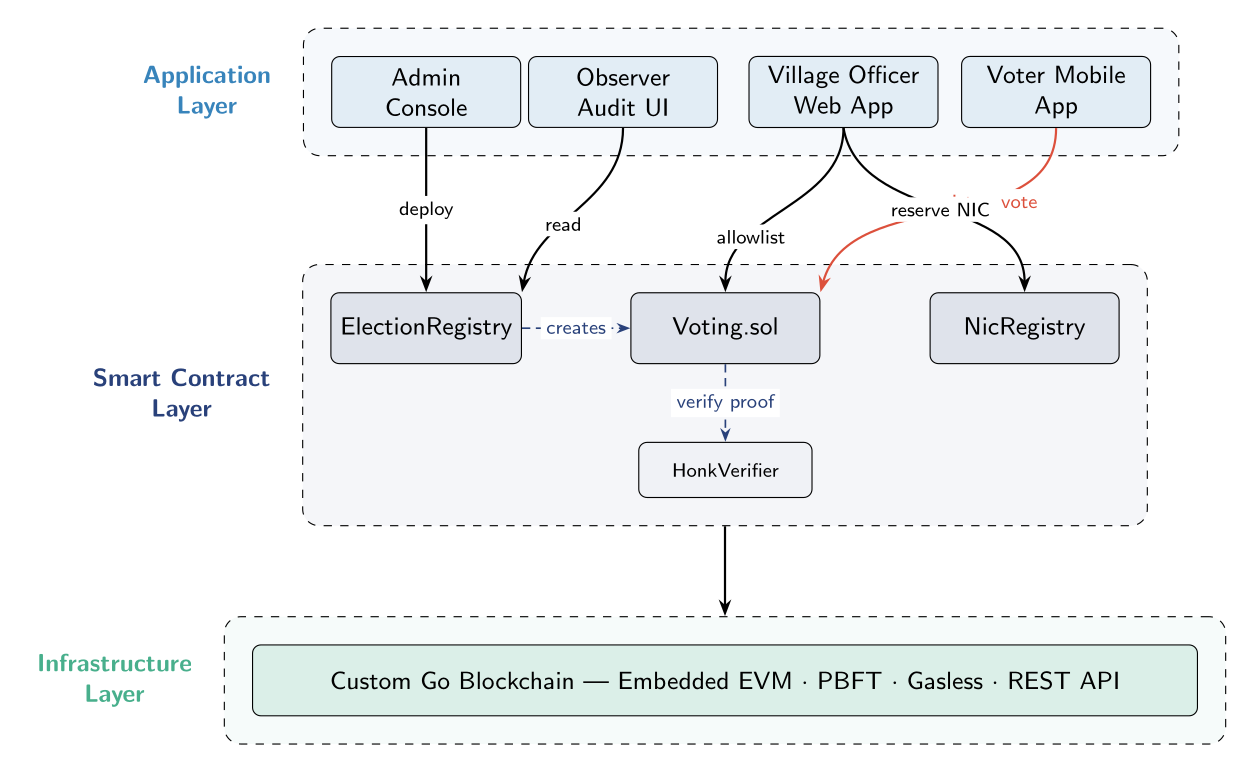
\includegraphics[width=0.85\textwidth]{Images/fig_system_architecture.png}
\caption{Four-layer system architecture showing the application layer, smart contract layer, blockchain infrastructure, and cryptographic foundation.}
\label{fig:system-architecture}
\end{figure}

\subsection{Layer 1: Application Layer}

The application layer provides user-facing interfaces for all system roles:

\begin{table}[H]
\centering
\caption{Application layer components and their target users.}
\label{tab:app-layer}
\begin{tabular}{|l|l|l|l|}
\hline
\textbf{Component} & \textbf{Technology} & \textbf{Users} & \textbf{Functions} \\
\hline
Mobile Voter App & React Native (Expo 54) & Citizens & Identity, Register, Vote, Verify \\
\hline
Admin Console & Next.js (Scaffold-ETH 2) & Election Authority & Division mgmt, Phase control \\
\hline
GN Portal & Next.js & Village Officers & Voter enrollment, NIC check \\
\hline
Results Dashboard & Next.js & Public/Observers & Live tallies, Division breakdown \\
\hline
Audit Interface & Next.js & Auditors & Proof verification, Tree rebuild \\
\hline
\end{tabular}
\end{table}

\subsection{Layer 2: Smart Contract Layer}

Four Solidity contracts implement the election logic:

\begin{table}[H]
\centering
\caption{Smart contract layer with deployment dependencies.}
\label{tab:contract-layer}
\begin{tabular}{|l|l|p{6cm}|}
\hline
\textbf{Contract} & \textbf{Depends On} & \textbf{Responsibility} \\
\hline
\texttt{HonkVerifier.sol} & None & ZK proof verification (auto-generated) \\
\hline
\texttt{Voting.sol} & HonkVerifier & Per-division election state machine \\
\hline
\texttt{ElectionRegistry.sol} & HonkVerifier, Voting & Division factory + national aggregation \\
\hline
\texttt{NicRegistry.sol} & None & Cross-division Sybil prevention \\
\hline
\end{tabular}
\end{table}

\begin{figure}[H]
\centering
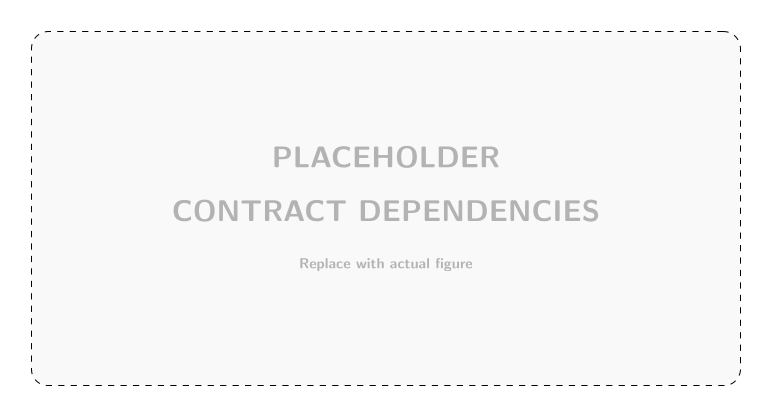
\includegraphics[width=0.85\textwidth]{Images/fig_contract_dependencies.png}
\caption{Contract dependency graph showing the deployment order and interaction patterns between the four smart contracts.}
\label{fig:contract-deps}
\end{figure}

\subsection{Layer 3: Blockchain Infrastructure}

A custom Go blockchain provides the execution environment:
\begin{itemize}
    \item Embedded go-ethereum EVM for Solidity execution
    \item PBFT consensus among election commission nodes
    \item BoltDB persistence for block storage
    \item REST API for application interaction
    \item Gasless execution model (no transaction fees)
    \item mTLS P2P communication between nodes
\end{itemize}

\subsection{Layer 4: Cryptographic Foundation}

The cryptographic layer provides the mathematical guarantees:
\begin{itemize}
    \item BN254 elliptic curve (scalar field $\mathbb{F}_r$, 254-bit security)
    \item Poseidon hash function (algebraically native to $\mathbb{F}_r$)
    \item UltraHonk proof system (no trusted setup, keccak transcript)
    \item LeanIMT incremental Merkle tree ($O(\log n)$ updates and proofs)
\end{itemize}

\section{Threat Model and Adversary Capabilities}

\subsection{Adversary Classes}

We consider three classes of adversaries with increasing capabilities:

\begin{definition}[External Adversary ($\mathcal{A}_{\text{ext}}$)]
An adversary who can observe all public blockchain data, intercept network traffic, and attempt to vote fraudulently. Cannot access voter devices or compromise system infrastructure.
\end{definition}

\begin{definition}[Infrastructure Adversary ($\mathcal{A}_{\text{infra}}$)]
An adversary who controls up to $f < n/3$ blockchain validator nodes, can observe all API traffic, and may attempt to manipulate the election state. Cannot access voter private keys.
\end{definition}

\begin{definition}[Coercing Adversary ($\mathcal{A}_{\text{coerce}}$)]
An adversary who can observe a voter during the voting process and demand proof of how they voted. May offer bribes or threaten consequences.
\end{definition}

\subsection{Trust Assumptions}

Our system makes the following minimal trust assumptions:
\begin{enumerate}
    \item The voter's device hardware is not compromised (TEE/Secure Enclave intact)
    \item At least $2n/3 + 1$ validator nodes are honest (PBFT threshold)
    \item The BN254 discrete logarithm assumption holds
    \item The Poseidon hash function is collision-resistant
    \item The voter performs the voting action in a private environment
\end{enumerate}

\subsection{Attack Surface Analysis}

\begin{table}[H]
\centering
\caption{Attack surface analysis with corresponding defenses.}
\label{tab:attack-surface}
\begin{tabular}{|p{3cm}|p{4cm}|p{5cm}|}
\hline
\textbf{Attack Vector} & \textbf{Adversary Capability} & \textbf{Defense Mechanism} \\
\hline
Double voting & Submit two votes for same election & Nullifier hash uniqueness (on-chain) \\
\hline
Voter impersonation & Obtain voter's commitment & Hardware keystore + biometric gate \\
\hline
Vote buying/selling & Voter proves how they voted & Burner wallet (unlinkable sender) \\
\hline
Ballot stuffing & Add unauthorized votes & ZK proof of Merkle membership \\
\hline
Vote modification & Change ballot after casting & Vote bound into ZK proof \\
\hline
Sybil attack & Register in multiple divisions & NicRegistry hashed-NIC check \\
\hline
Front-running & Observe proof, change vote & Vote-binding in circuit \\
\hline
Replay attack & Resubmit valid proof & Nullifier consumed on-chain \\
\hline
State rollback & Revert blockchain state & PBFT finality (no reorgs) \\
\hline
Admin abuse & Authority manipulates results & Public verifiability + E2E audit \\
\hline
\end{tabular}
\end{table}

\section{Security Properties}

\subsection{Formal Security Theorem}

\begin{theorem}[Voter--Ballot Unlinkability]
\label{thm:unlinkability}
Under the BN254 discrete logarithm assumption and the collision resistance of Poseidon, for any probabilistic polynomial-time adversary $\mathcal{A}$ with access to the complete blockchain state:
\begin{equation}
\Pr\left[\mathcal{A}(\text{chain}, \text{proofs}, \text{nullifiers}) \to (\text{Voter}_i, \text{Ballot}_j)\right] \leq \frac{1}{|\mathcal{V}|} + \text{negl}(\lambda)
\end{equation}
where $|\mathcal{V}|$ is the number of registered voters and $\lambda$ is the security parameter.
\end{theorem}

\begin{proof}[Proof Sketch]
The proof proceeds by reduction to the zero-knowledge property of UltraHonk:
\begin{enumerate}
    \item The ZK proof reveals no information about the prover's identity (zero-knowledge).
    \item The Merkle path is hidden (private input), preventing leaf identification.
    \item The nullifier hash is a one-way function of the secret nullifier.
    \item The vote is submitted from a fresh burner wallet with no prior transaction history.
    \item Therefore, the adversary's view is computationally indistinguishable regardless of which voter cast which ballot.
\end{enumerate}
\end{proof}

\subsection{Double-Vote Prevention}

\begin{property}[Uniqueness]
Each registered voter can cast exactly one valid vote per election:
\begin{equation}
\forall v \in \mathcal{V}: |\{b \in \text{Ballots} : \text{nullifier}(b) = \Poseidon_1(r_v)\}| \leq 1
\end{equation}
\end{property}

This is enforced by the on-chain nullifier set: \texttt{s\_nullifierHashes[electionId][hash] = true}. Once a nullifier hash is consumed, any subsequent proof using the same nullifier is rejected.

\subsection{Eligibility Soundness}

\begin{property}[Eligibility]
Only voters whose commitment is in the Merkle tree can generate a valid proof:
\begin{equation}
\text{Honk.Verify}(\pi, x) = \text{true} \implies \exists \text{ leaf } l \in \text{Tree}(root) : l = \Poseidon_2(r, s)
\end{equation}
\end{property}

This follows from the soundness of the UltraHonk proof system---no polynomial-time adversary can forge a proof of Merkle membership for a commitment not in the tree.

\section{Election Phase State Machine}

The election lifecycle is modeled as a deterministic state machine with four phases:

\begin{figure}[H]
\centering
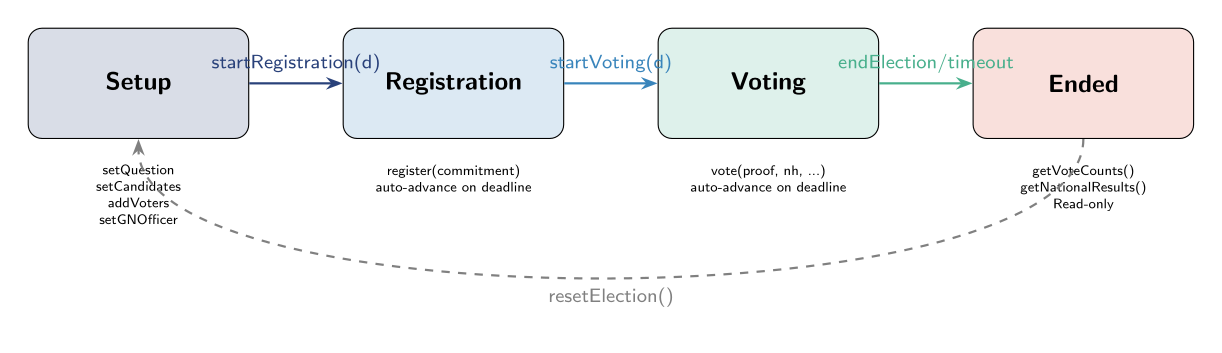
\includegraphics[width=0.85\textwidth]{Images/fig_phases.png}
\caption{Election phase state machine showing transitions, conditions, and automatic deadline-based advancement.}
\label{fig:phases}
\end{figure}

\subsection{Phase Definitions}

\begin{enumerate}
    \item \textbf{Setup Phase}: Administrator configures the election (question, candidates, voter allowlist, GN officer assignment). No time pressure; manual transition.
    
    \item \textbf{Registration Phase}: Allowlisted voters register their cryptographic commitments to the Merkle tree. Deadline-bounded; auto-advances to Voting when \texttt{registrationEndTime} passes.
    
    \item \textbf{Voting Phase}: Registered voters generate ZK proofs and cast anonymous ballots. Deadline-bounded; auto-advances to Ended when \texttt{votingEndTime} passes.
    
    \item \textbf{Ended Phase}: Election is concluded. Results are final and publicly readable. No further state changes permitted.
\end{enumerate}

\subsection{Transition Rules}

\begin{table}[H]
\centering
\caption{Phase transition rules with authorization and conditions.}
\label{tab:transitions}
\begin{tabular}{|l|l|l|p{5cm}|}
\hline
\textbf{Transition} & \textbf{Trigger} & \textbf{Auth} & \textbf{Conditions} \\
\hline
Setup $\to$ Registration & \texttt{startRegistration(d)} & Owner & Duration $> 0$, candidates set \\
\hline
Registration $\to$ Voting & \texttt{startVoting(d)} & Owner & Duration $> 0$, or auto after deadline \\
\hline
Voting $\to$ Ended & \texttt{endElection()} & Owner & Or auto after deadline \\
\hline
Any $\to$ Setup & \texttt{resetElection()} & Owner & Bumps electionId \\
\hline
\end{tabular}
\end{table}

The \texttt{\_maybeAdvancePhase()} modifier automatically checks deadlines on every state-mutating call, ensuring that phase transitions occur even without explicit admin action.

\section{Cryptographic Protocol Design}

\subsection{Commitment Scheme}

During registration, each voter generates a cryptographic commitment that binds their identity to the election without revealing it:

\begin{equation}
\text{commitment} = \Poseidon_2(\text{nullifier}, \text{secret})
\end{equation}

where:
\begin{itemize}
    \item $\text{nullifier} \xleftarrow{\$} \mathbb{F}_r$: random field element, stored in hardware keystore
    \item $\text{secret} \xleftarrow{\$} \mathbb{F}_r$: random field element, stored in hardware keystore
    \item The commitment is a deterministic function of both secrets
\end{itemize}

The commitment serves as the voter's ``ticket'' to the election---it is inserted as a leaf in the Merkle tree during registration.

\subsection{Nullifier Mechanism}

The nullifier provides double-vote prevention while maintaining anonymity:

\begin{equation}
\text{nullifier\_hash} = \Poseidon_1(\text{nullifier})
\end{equation}

\textbf{Key properties}:
\begin{itemize}
    \item Deterministic: same nullifier always produces same hash (prevents double-voting)
    \item One-way: hash cannot be inverted to recover the nullifier (preserves privacy)
    \item Unique per voter: different voters have different nullifiers (distinguishable rejections)
\end{itemize}

\subsection{Merkle Membership Proof}

The voter proves their commitment is in the tree by providing the authentication path:

\begin{equation}
\text{verify\_path}(\text{commitment}, \text{siblings}[0..d-1], \text{index\_bits}[0..d-1]) \stackrel{?}{=} \text{root}
\end{equation}

The path traversal uses little-endian bit decomposition of the leaf index:
\begin{align}
h_0 &= \text{commitment} \\
h_{i+1} &= \begin{cases}
\Poseidon_2(h_i, \text{siblings}[i]) & \text{if } \text{index\_bits}[i] = 0 \\
\Poseidon_2(\text{siblings}[i], h_i) & \text{if } \text{index\_bits}[i] = 1
\end{cases}
\end{align}

The final computed hash $h_d$ must equal the published Merkle root.

\subsection{Complete Protocol Flow}

\begin{algorithm}[H]
\caption{Complete Voting Protocol}
\label{alg:protocol}
\begin{algorithmic}[1]
\STATE \textbf{Registration Phase:}
\STATE Voter generates $(\text{nullifier}, \text{secret}) \xleftarrow{\$} \mathbb{F}_r^2$
\STATE Voter computes $\text{commitment} = \Poseidon_2(\text{nullifier}, \text{secret})$
\STATE Voter submits $\text{register}(\text{commitment})$ to division contract
\STATE Contract inserts commitment into LeanIMT tree
\STATE
\STATE \textbf{Voting Phase:}
\STATE Voter retrieves Merkle path from chain state
\STATE Voter constructs witness $w = (\text{nullifier}, \text{secret}, \text{index}, \text{siblings})$
\STATE Voter constructs public inputs $x = (\Poseidon_1(\text{nullifier}), \text{root}, \text{vote}, \text{depth})$
\STATE Voter generates proof: $\pi \leftarrow \text{UltraHonk.Prove}(x, w)$
\STATE Voter creates burner wallet (fresh keypair)
\STATE Voter funds burner via faucet/paymaster
\STATE Voter submits $\text{vote}(\pi, \text{nullifier\_hash}, \text{root}, \text{vote}, \text{depth})$ from burner
\STATE Contract verifies: $\text{HonkVerifier.verify}(\pi, [x_1, x_2, x_3, x_4])$
\STATE Contract checks: nullifier\_hash not in used set
\STATE Contract increments vote count, records nullifier
\end{algorithmic}
\end{algorithm}

\section{Multi-Division Architecture}

\subsection{Sri Lanka's Electoral Structure}

Sri Lanka's electoral system comprises 22 electoral districts containing 160 polling divisions. Our system models this hierarchy on-chain:

\begin{figure}[H]
\centering
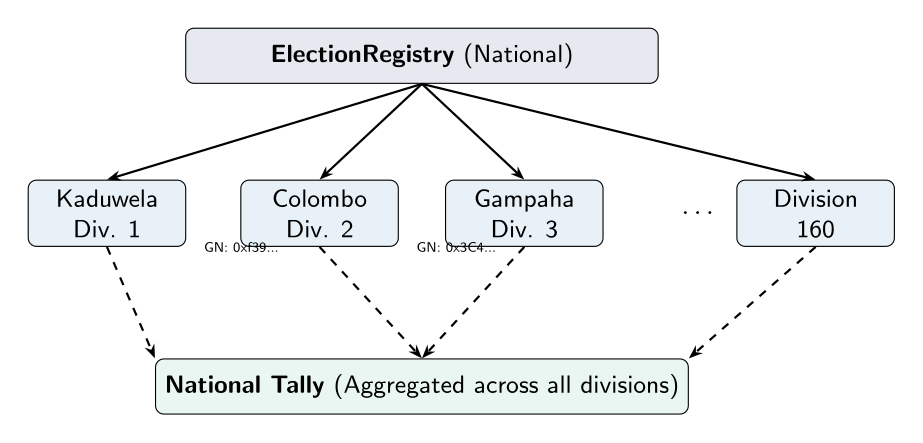
\includegraphics[width=0.85\textwidth]{Images/fig_divisions.png}
\caption{Multi-division architecture: ElectionRegistry deploys 160 independent Voting contracts with national aggregation.}
\label{fig:divisions}
\end{figure}

\subsection{Factory Pattern Design}

The \texttt{ElectionRegistry} contract implements the factory pattern:

\begin{lstlisting}[language=Java, caption={ElectionRegistry factory pattern (simplified).}]
function createDivision(string name) external onlyOwner
    returns (uint256 divisionId, address votingContract)
{
    Voting newVoting = new Voting(i_verifier, msg.sender);
    divisions.push(Division({
        name: name,
        votingContract: address(newVoting),
        gnOfficer: address(0),
        active: true
    }));
    divisionId = divisions.length - 1;
    votingContract = address(newVoting);
}
\end{lstlisting}

\textbf{Design decisions}:
\begin{itemize}
    \item Each division gets an independent \texttt{Voting.sol} instance (isolation)
    \item All share a single \texttt{HonkVerifier} (gas efficiency---deploy once, verify many)
    \item GN officers are assigned per-division (delegated administration)
    \item National aggregation is read-only (no cross-division write dependencies)
\end{itemize}

\subsection{National Result Aggregation}

The registry provides national-level views by summing across all active divisions:

\begin{equation}
\text{NationalVotes}[c] = \sum_{d \in \text{ActiveDivisions}} \text{Division}_d.\text{voteCounts}[c]
\label{eq:national-agg}
\end{equation}

This computation is performed on-chain as a view function (no gas cost), enabling any observer to independently verify the national tally.

\section{Five-Layer Fraud Prevention}

Our system implements defense in depth through five independent fraud prevention layers:

\begin{table}[H]
\centering
\caption{Five-layer fraud prevention architecture.}
\label{tab:fraud-layers}
\begin{tabular}{|c|l|p{4cm}|p{4cm}|}
\hline
\textbf{Layer} & \textbf{Name} & \textbf{Mechanism} & \textbf{Prevents} \\
\hline
1 & Identity Gate & Hardware keystore + biometric & Device-level impersonation \\
\hline
2 & Eligibility Proof & ZK Merkle membership & Unauthorized ballot casting \\
\hline
3 & Uniqueness Enforcement & On-chain nullifier set & Double voting \\
\hline
4 & National De-duplication & NicRegistry (hashed NIC) & Cross-division Sybil \\
\hline
5 & Cryptographic Binding & Vote in proof statement & Front-running, modification \\
\hline
\end{tabular}
\end{table}

\subsection{Layer 1: Identity Gate}

Before any election-related action, the mobile app requires biometric authentication:
\begin{itemize}
    \item Voter's private key stored in \texttt{expo-secure-store} with \texttt{requireAuthentication: true}
    \item Device's Trusted Execution Environment (TEE) or Secure Enclave protects key material
    \item Even with physical device access, keys cannot be extracted without biometric enrollment
\end{itemize}

\subsection{Layer 2: ZK Eligibility Proof}

The zero-knowledge proof demonstrates that the voter's commitment exists in the Merkle tree without revealing which commitment is theirs. A voter who was never registered (no leaf in tree) cannot produce a valid proof.

\subsection{Layer 3: Nullifier Uniqueness}

Each voter's nullifier produces a unique, deterministic hash. The contract maintains a mapping:
\begin{lstlisting}[language=Java, caption={Nullifier uniqueness enforcement.}]
mapping(uint256 electionId => mapping(bytes32 => bool)) s_nullifierHashes;

// In vote():
if (s_nullifierHashes[s_electionId][_nullifierHash])
    revert NullifierHashAlreadyUsed(_nullifierHash);
s_nullifierHashes[s_electionId][_nullifierHash] = true;
\end{lstlisting}

\subsection{Layer 4: NIC Registry}

The \texttt{NicRegistry} stores hashed National Identity Card numbers:
\begin{equation}
\text{nicHash} = \Poseidon(\text{NIC\_number}, \text{SERVER\_PEPPER})
\end{equation}

This prevents a voter from registering in multiple divisions using the same NIC. The server pepper ensures that the NIC hash cannot be computed without the election authority's secret, preventing brute-force enumeration.

\subsection{Layer 5: Vote Binding}

The candidate index is a public input to the ZK circuit:
\begin{lstlisting}[language=Java, caption={Vote binding in the Noir circuit.}]
// Circuit constrains: vote is bound into the proof
vote_bits: [u1; 8] = vote.to_le_bits();
// The proof is only valid for this specific candidate index
\end{lstlisting}

An adversary who intercepts the proof cannot substitute a different vote---the proof is cryptographically bound to the candidate index.

\section{Voting.sol State Machine Design}

\begin{figure}[H]
\centering
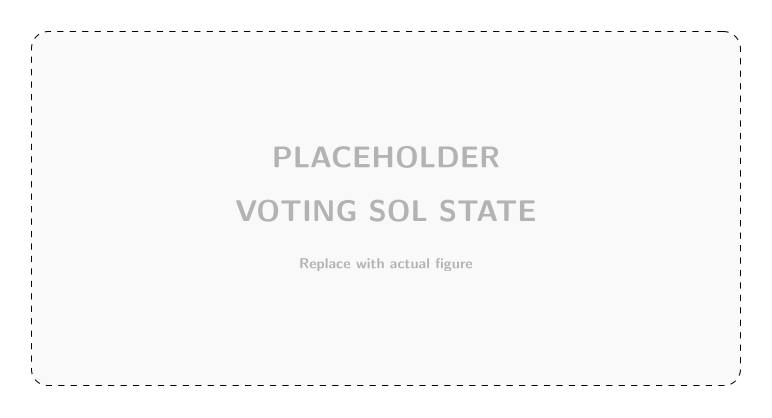
\includegraphics[width=0.85\textwidth]{Images/fig_voting_sol_state.png}
\caption{Detailed state diagram of Voting.sol showing all state variables, transitions, and per-election isolation through electionId keying.}
\label{fig:voting-state}
\end{figure}

\subsection{Per-Election Isolation}

A critical design choice is keying all mutable state by \texttt{electionId}:

\begin{lstlisting}[language=Java, caption={Election-keyed state isolation.}]
// All per-election state is isolated
mapping(uint256 => mapping(address => bool)) s_voters;
mapping(uint256 => mapping(address => bool)) s_hasRegistered;
mapping(uint256 => mapping(uint256 => bool)) s_commitments;
mapping(uint256 => mapping(bytes32 => bool)) s_nullifierHashes;
mapping(uint256 => mapping(uint256 => uint256)) s_voteCounts;
mapping(uint256 => IncrementalTreeData) s_trees;
\end{lstlisting}

When \texttt{resetElection()} is called, the \texttt{electionId} increments. All previous state remains intact (for audit) but is no longer accessible to current-election operations. This enables contract reuse across multiple election cycles without redeployment.

\section{Data Flow Architecture}

The complete data flow from voter action to on-chain state change follows this path:

\begin{enumerate}
    \item \textbf{User Action}: Voter interacts with mobile app
    \item \textbf{Local Cryptography}: Secrets retrieved from keystore, commitment/proof generated
    \item \textbf{Network Transport}: REST API call to custom blockchain node
    \item \textbf{API Handler}: Go HTTP handler validates format, applies rate limits
    \item \textbf{EVM Execution}: Embedded go-ethereum EVM executes Solidity bytecode
    \item \textbf{State Transition}: Contract logic validates and updates state
    \item \textbf{Block Commit}: PBFT consensus finalizes the state change
    \item \textbf{Persistence}: BoltDB stores the committed block
    \item \textbf{Event Emission}: Blockchain events propagate to listening clients
\end{enumerate}

\section{Summary}

This chapter has established the architectural foundation of our privacy-preserving voting system. The four-layer design provides clear separation of concerns while the five-layer fraud prevention ensures defense in depth. The formal security theorem (Theorem~\ref{thm:unlinkability}) provides mathematical assurance of voter--ballot unlinkability. The multi-division factory pattern faithfully models Sri Lanka's 160-division electoral structure. Chapter~\ref{ch:methodology} next describes the development methodology and the iterative journey from initial prototypes to the final architecture presented here.
